\documentclass[dvipdfmx]{jsarticle}
\usepackage[dvipdfmx]{graphicx}
\graphicspath{{ピクチャ/}}
\usepackage{otf}
\usepackage[dvipdfmx]{graphicx}
\usepackage{amsmath,amssymb}
\usepackage{url}
\begin{document}

\title{\huge 英語論文セミナー 第二回}
\date{}
\maketitle

\begin{flushright}
2022/5/30\\
学籍番号:s0319007\\
氏名:上野智也\\
\end{flushright}

\section{課題}

\subsection{アンビルセルの大きさ}

supplymentにアンビルセルの大きさが書かれていなかったため、調べた値を以下に示す。

  

・株式会社システムズエンジニアリングの高圧ダイアモンドアンビルセル

アンビル面サイズ 0.8mm 高さ 14mm(ねじ除く)

  

・東京大学高木研究室10GPa級対向アンビル超高圧セル

セルサイズ$\phi$29$\times$42mm

セルサイズ$\phi$22$\times$34mm

  

論文及びsupplymentを読むと、今回使用した試料の大きさは、横の長さが約80~100$\mu$m、厚さが約80$\mu$mの不規則な五角形である。したがって、試料に比べてアンビルセルはとても大きいことが分かる。

\newpage

\subsection{BaFe$_2$(As$_{1-x}$P$_x$)$_2$の結晶構造}

本論文で用いている物質BaFe$_2$(As$_{1-x}$P$_x$)$_2$の結晶構造は以下に示す通りである。

\begin{figure}[h]
\centering
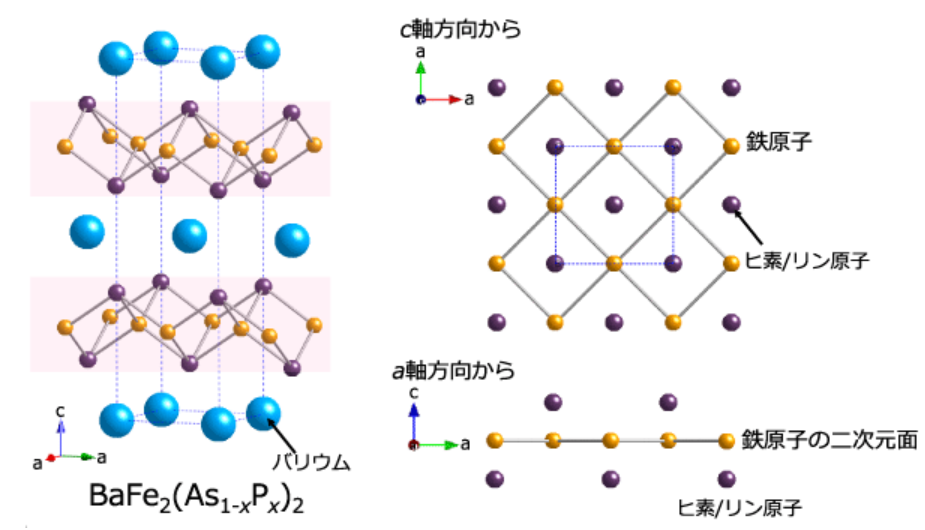
\includegraphics[width=13cm]{structure.png}
\caption{BaFe$_2$(As$_{1-x}$P$_x$)$_2$の結晶構造}
\end{figure}%

\section{本文}

図2Aに示すようなパルスシーケンスを用いてODMRデータを収集した。弱い磁場で温めてからデータを取ったので、超伝導に伴う反磁性も探ることができた。マイクロ波やレーザー照射による加熱を避けるため、測定に伴う超伝導状態への摂動を緩和する測定手順を考案した(20)。図2のB~Dに、3つのダイヤモンド粒子の8.3 kbarにおける代表的なODMRスペクトルを示す。このときの試料温度(~7.7 K)はTc(8.3 kbarにおいて~20.4 K、ゼロ磁場における交流磁化率を用いて決定)よりはるかに低い(20)。ODMRスペクトルは、異なる分裂を示す。これは周りの磁場によるゼーマン効果による分裂である。したがって、ODMRスペクトルは磁場を検出する手段を提供する。NV$_C$のゼーマン分裂(~64 MHz)は、T<TcではNV$_E$のゼーマン分裂(~658 MHz)の10倍小さいが、T>Tcではその差ははるかに小さくなる(図2G)。NV$_C$の温度を変えたときのODMRスペクトルを図2Eに示し、そこから分裂を抽出してプロットしたのが図2Fである。温められると、分裂の度合いは最初はほぼ一定であるが、約17K以降顕著に増加する。21K以降は再び分裂が一定となる。超伝導との関連性を示すため、同じ実験で交流帯磁率データを追加収集した。これは、実験構成にモジュレーションコイルを追加したことで可能となった。マイクロコイルをピックアップコイルとして用いると、同じ温度で超伝導転移を意味する交流磁化率の急激な低下(25, 26)が検出された(図2F)。2つの方法は、Tcの測定においてよく一致した。

局所磁場分布の変化は、NV$_E$とNV$_F$の分割の温度変化でも確認できる(図2G)。NV$_C$の挙動とは逆に、NV$_E$は温めると分割の度合いが小さくなる。参考までに、NV$_F$の分裂は温度に対してほぼ一定であり、これはNV$_F$が超伝導体から遠く離れているためであり、全磁場が変化していないと理解することができる。これらの観測結果は、先に説明した超伝導に伴う反磁性からの予想とよく一致する。線幅やESR線全体のコントラストに顕著な変化は見られなかった。これは、超伝導に伴う反磁性によって引き起こされる磁場勾配に比べ、ダイヤモンド粒子の大きさがはるかに小さかったためである。試料の大きさが有限であり、ダイヤモンド粒子と試料の間隔が狭いため、残留磁場があり、低温でのNV$_C$のゼーマン分裂は〜64MHzであった。また、3つのダイヤモンド粒子は磁場に対してランダムな配向をしているため、試料が常伝導状態でもゼーマン分裂に違いが見られた。

本技術の大きなメリットの一つが、図2Hに示されている。前述のように、ある NV の中心に対する磁場の横方向と縦方向の成分は、その ODMR スペクトルから計算することができる。これにより、磁場のベクトルを再構築する手段を得ることができる。試料が常伝導状態であれば、NV中心の向きは、試料のc軸に沿った印加磁場方向に対して較正することができる。これにより、c軸に沿った有効磁場ベクトルが得られ、温度の関数として追跡することができる(20)。これらの考察から、NV$_C$、NV$_E$、NV$_F$が8.3 kbarで感じる実効磁場ベクトルを決定した。NV$_C$の場合、超伝導状態に入ると磁場ベクトルは短くなり、垂直方向から離れる方向に傾く。これは、NV$_C$が試料の上部にあり、超伝導に伴う反磁性によって磁束線が試料の周囲で曲がっていることと矛盾しない。しかし、NV$_E$の場合、超伝導状態では磁場ベクトルは長くなり、わずかに傾くだけである。ここでも、NV$_E$が試料の脇に位置しているため、マイスナー状態では磁束線が垂直のまま密になることと矛盾しない。最後に、NV$_F$によって感知される磁場ベクトルは、NV$_E$とNV$_C$の挙動とは全く対照的に、超伝導相転移の間、実質的に一定である。極端な条件下で、完全なベクトル情報を空間分解能で収集できることは、この技術の重要な進歩の一つである。 

\begin{thebibliography}{9}
\item 株式会社 システムズエンジニアリング 「高圧ダイアモンドアンビルセル」 閲覧日2022/5/26

URL:\url{https://www.systems-eng.co.jp/dcms_media/other/diaanvil_datasheet.pdf}

\item 東京大学高木研究室 「10GPa級対向アンビル超高圧セル」 閲覧日2022/5/26

\item spring-8 「鉄原子を含む高温超伝導体の仕組みを解くカギ「電子のネマティック液晶状態」を発見」 2012年 
閲覧日2022/5/26

URL:\url{http://www.spring8.or.jp/ja/news_publications/press_release/2012/120621/}
  
\end{thebibliography}


\newpage

\begin{figure}[h]
\centering
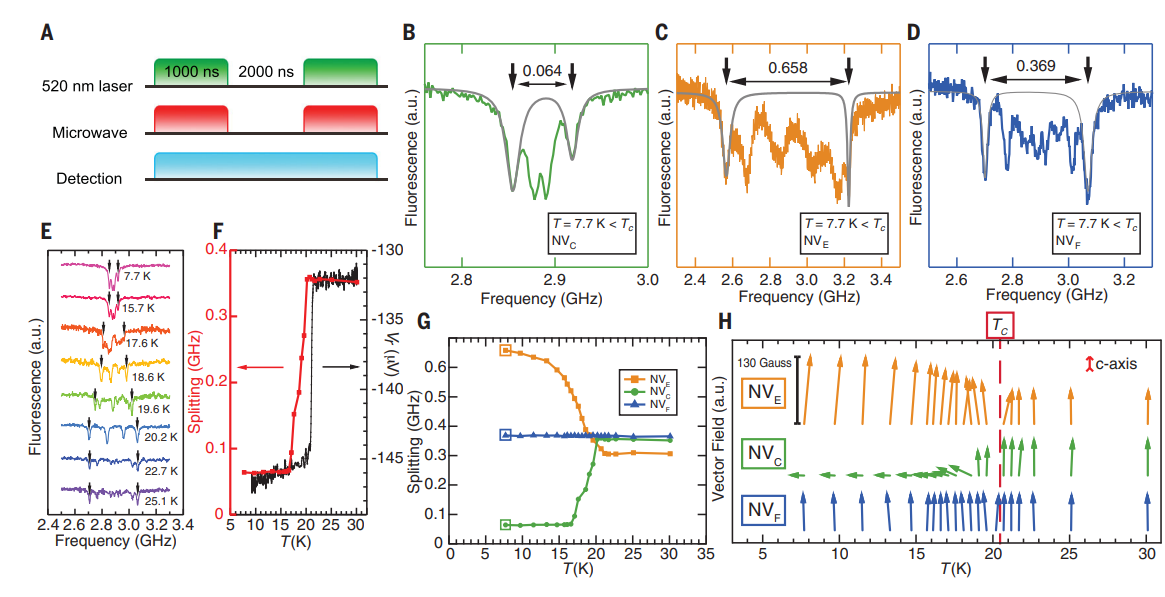
\includegraphics[width=16cm]{Fig.2.png}
\caption{図2 8.3 kbarにおけるBaFe$_2$(As$_{0.59}$P$_{0.41}$)$^2$をNVセンターを用いて感知した超伝導に伴う反磁性}
\end{figure}%

図2のステートメント

(A)ODMRを用いたパルスシーケンス

(B~D)7.7Kにおけるそれぞれのダイヤモンド粒子のODMRスペクトル。ゼーマン分裂を決定するためのローレンツフィットは、灰色の線で示されている。

(E)違う温度でのNV$_C$中のNVのODMRスペクトル

(F)転移温度Tcの決定におけるODMR法(赤)と交流磁化率法(黒)の比較。

(G)NV$_C$、NV$_E$、NV$_F$のNVセンターに対するゼーマン分裂の温度による変化。

(H)NV$_C$、NV$_E$、NV$_F$のNVセンターが感じる局所磁場ベクトルの、超伝導相転移に伴う変化。縦方向はサンプルのc軸である。ODMR測定は、レーザー出力10mW、マイクロ波ピーク出力30mWで行われた。試料のc軸に沿って68Gの外部磁場が印加された。

\newpage

\section{用語}

・ゼーマン効果

原子から放出される電磁波のスペクトルにおいて、磁場が無いときには単一波長であったスペクトル線が、原子を磁場中においた場合には複数のスペクトル線に分裂する現象である。

縮退していたエネルギー準位が磁場の印加によって分裂したともいえる。

  

・交流磁化率

交流磁場をかけた時の応答として現れる動的な磁化率を交流磁化率と呼ぶ。

  

・ローレンツ関数

分光分析においてスペクトルの波形分離の際、孤立スペクトルの形状、バックグラウンドの形状を仮定するときに用いる関数。 この関数をもちいてバックグラウンドの前処理やスペクトル強度のフィッティングを行う。

以下の形で表される。

\begin{equation}
\displaystyle f(x)=A\frac{w^2}{4(x-x_0)^2+w^2}
\end{equation}

ただし、$A$は強度、$x_0$は位置、$w$は幅である。

  

・ピックアップコイル

磁場の時間変化を求めるためのコイル。

  

・G(ガウス)

磁場の強さの単位。1G=10$^{-4}$T(テスラ)。地磁気は0.5G











\end{document}